\documentclass[master=cws,masteroption=vs]{kulemt}
\usepackage{listings}
\usepackage{bytefield}
\usepackage{color}
\setup{% Remove the "%" on the next line when using UTF-8 character encoding
  inputenc=utf8,
  title={Borrowed Capabilities},
  author={Thijs Vercammen},
  promotor={Prof.\,dr.\,ir.\ Dominique Devriese\and Prof.\,dr.\,ir.\ Frank Piessens},
  assessor={Ir.\,Kn. Owsmuch\and K. Nowsrest},
  assistant={Ir.\ Thomas Van Strydonck}}
% Remove the "%" on the next line for generating the cover page
%\setup{coverpageonly}
% Remove the "%" before the next "\setup" to generate only the first pages
% (e.g., if you are a Word user).
%\setup{frontpagesonly}

% Choose the main text font (e.g., Latin Modern)
\setup{font=lm}

% If you want to include other LaTeX packages, do it here. 

% Finally the hyperref package is used for pdf files.
% This can be commented out for printed versions.
\usepackage[pdfusetitle,colorlinks,plainpages=false]{hyperref}

%%%%%%%
% The lipsum package is used to generate random text.
% You never need this in a real master's thesis text!
\IfFileExists{lipsum.sty}%
 {\usepackage{lipsum}\setlipsumdefault{11-13}}%
 {\newcommand{\lipsum}[1][11-13]{\par And some text: lipsum ##1.\par}}
%%%%%%%

%\includeonly{chap-n}
\begin{document}

\begin{preface}
  I would like to thank everybody who kept me busy the last year,
  especially my promoter and my assistants. I would also like to thank the
  jury for reading the text. My sincere gratitude also goes to my wive and
  the rest of my family.
\end{preface}

\tableofcontents*

\begin{abstract}
  The \texttt{abstract} environment contains a more extensive overview of
  the work. But it should be limited to one page.

  \lipsum[1]
\end{abstract}

% A list of figures and tables is optional
%\listoffigures
%\listoftables
% If you only have a few figures and tables you can use the following instead
\listoffiguresandtables
% The list of symbols is also optional.
% This list must be created manually, e.g., as follows:
\chapter{List of Abbreviations and Symbols}
\section*{Abbreviations}
\begin{flushleft}
  \renewcommand{\arraystretch}{1.1}
  \begin{tabularx}{\textwidth}{@{}p{12mm}X@{}}
    LoG   & Laplacian-of-Gaussian \\
    MSE   & Mean Square error \\
    PSNR  & Peak Signal-to-Noise ratio \\
  \end{tabularx}
\end{flushleft}
\section*{Symbols}
\begin{flushleft}
  \renewcommand{\arraystretch}{1.1}
  \begin{tabularx}{\textwidth}{@{}p{12mm}X@{}}
    42    & ``The Answer to the Ultimate Question of Life, the Universe,
            and Everything'' according to \cite{h2g2} \\
    $c$   & Speed of light \\
    $E$   & Energy \\
    $m$   & Mass \\
    $\pi$ & The number pi \\
  \end{tabularx}
\end{flushleft}

% Now comes the main text
\mainmatter

\chapter{Introduction}
\label{cha:intro}
For many years computer programs have been plagued by vulnerabilities that can be exploited in order to gain control over the execution of a program.
Several classes of these vulnerabilities arise from bugs in the source code and are related to low level control over memory.
Spatial memory issues are vulnerabilities that arise from accessing memory that is outside of the bounds that are supposed to be accessed.
Temporal memory issues on the other hand arise from accessing memory after the reference to that memory is supposed to have been invalidated.
Some famous examples of spatial and temporal memory issues are buffer overflows and use after free whereby an attacker can write to memory that is not supposed to be written to\tomi{add some references whenever you make claims like this; you have very few references atm}.

Over the past decades, several solutions to these issues have been presented and implemented.
One of the most popular solution is the usage of memory safe programming languages that deny the programmer low level access to the memory\tomi{some example refs}.
Instead, the memory is managed by a language runtime and deallocated by a garbage collector.
This solution, however, has a significant performance impact and is thus not applicable to performance sensitive programs such as kernels, browsers and low level system libraries.
These types of programs remain vulnerable and are often a vector for malware to gain control over a system.
A class of devices that are especially vulnerable to these issues are embedded devices, since they have constrained resources and programmers require low level memory management features to gain reasonable performance.
With the advent of the Internet of Things (IoT), these embedded devices are expected to increase in number dramatically\tomi{ref}.

Over the past few years programming languages with strong type systems have gained renewed attention as a way to mitigate these issues and improve security\tomi{strong claim; prove with ref or weaken}.
One of the most popular of these is the Rust programming language\tomi{ref}.
Rust offers a number of security features, but in this thesis we will focus on Rust's ownership and borrowing system.
This system limits what a programmer can do with references to an object in memory, ensuring that memory is always accessed in a safe manner, and statically guaranteeing thread safety.
One of the most important principles of this system is the principle of ``aliasing XOR mutability'' which means that references to a resource in memory are either allowed to mutate the resource or are read-only and can be copied, but not both.
This prevents concurrent write accesses and concurrent read and write access to a resource in memory, which ensures the absence of things like data races.

However, when a Rust program is compiled, it is usually converted into an unsafe assembly language that does not have any of these safety guarantees\tomi{refer to some secure compilation paper}.
This might, for example, open the programs up to attacks on the assembly level if they are linked with libraries that are not written in a programming language with the same safety guarantees.
In this thesis we explore an extension to the capability machine architecture CHERI in order to provide support on the assembly level for the safety guarantees that the Rust programming language offers.

Hardware capabilities are unforgeable pointers that represent authority over a region of memory.
They are comparable to software fat pointers in that they enforce bounds checking and hold permissions that specify how a region of memory can be used.
This model is very effective at combating spatial memory issues, but is less suited to enforce the temporal memory safety guarantees offered by languages with strong type systems.
Nevertheless, CHERI does offer some hardware primitives that software can build upon to strengthen their defense against temporal memory issues.
In this thesis we will add a new type of capability called \textit{borrowed capability}.
This new type of capability is designed to mimic Rust's ownership and borrowing system, but it could be seen in a wider context as an addition to the types of revocation that are already offered by CHERI.

In summary, the goal of this thesis is to design an extension to the CHERI architecture that offers the same memory and thread safety guarantees as the Rust programming language.
\tomi{Mention section numbers in explanation below, since you're going over the sections anyways + update to include discussion section}
To test our design, we will implement it in the Sail specification language, extend the LLVM project to create an assembler for our extension and run test programs on the emulator generated by Sail.
We start off by giving background information about Rust and CHERI as well as information about RISC-V and the Sail language which will be essential for the implementation of our design.
Next, we provide an overview of our design, followed by the details of its implementation in Sail and the details of the LLVM extension.
Finally, we will evaluate our design by constructing a number of assembly example programs and reason about how well they mimic the Rust ownership and borrowing system.

%%% Local Variables: 
%%% mode: latex
%%% TeX-master: "thesis"
%%% End: 

\chapter{Literature Review}
\label{cha:litrev}
The topic of this thesis lies at the intersection of multiple different fields including programming languages, capability machines, formal software verification and instruction set architecture (ISA) design. Understanding this thesis requires background knowledge of each of these individual subjects.

\section{The Rust programming language}
\label{sec:rustbackground}
Rust is a relatively new programming language that aims to provide the high performance associated with other low-level programming languages such as C and C++ while simultaneously preventing a number of classes of bugs related to memory and thread safety that typically arise due to the low-level resource management features necessary to achieve such high performance.
Rust accomplishes this at compile time by statically checking if the source code satisfies the rules of Rust's strong ownership-based type system.
Because these rules are conservative and might reject correct programs, Rust provides an \textit{unsafe} mode in which some of these rules do not need to be satisfied.
Since this thesis is about the safety Rust provides, we only consider \textit{safe} Rust in this section.

\subsection{Ownership}
Central to Rust's resource management model is the concept of ownership.
When a value gets created, ownership of that value will be assigned to a variable.
This value stays valid until its owner goes out of scope after which it cannot be used anymore.
Ownership of a value can be transferred to another variable, when this happens the value cannot be accessed anymore through the original variable.
This is illustrated in listing \ref{code:move} which fails to compile because \textit{a} gets accessed after its value has been moved to \textit{b}.
\begin{lstlisting}[language=Rust,frame=single,caption=Moving a variable,label=code:move]
fn main() {
  let a = String::from("This is a heap allocated string");
  let b = a;
  println!("{}", a);
}
\end{lstlisting}

\subsection{Borrowing}
\label{subsec:borrowing}
As mentioned, Rust follows the principle of ``aliasing XOR mutation'' to prevent a number of bugs related to memory safety and data races.
The borrowing system has a set of rules that enforces this principle.
A value can be borrowed by variables other than its owner, giving those variables temporarily the right to use the value.
There are two types of borrows: a mutable borrow and an immutable (or shared) borrow. 

A mutable borrow allows the borrowing variable to both read and mutate the contents of the value.
To prevent multiple variables mutating the same value at the same time and to prevent variables from reading a value that is being altered, the owner temporarily loses its right to access or lend the value while a mutable borrow is in scope.
As a result, only the borrowing variable is allowed to access the value while a mutable borrow exists.

A shared borrow only allows a borrowing variable to read the contents of the value.
While a shared borrow is in scope, the owner cannot mutate or mutably lend the value anymore.
It is however allowed to read the value and immutably lend the value again.
This means that an unlimited amount of shared borrows can read a value at the same time, but it cannot be mutated while any of those shared borrows exist.

Listing \ref{code:borrowexample} shows a simple program that creates a mutable variable \textit{x}, borrows it mutably and increments the value through that borrow 
Then, after the mutable borrow has ended, the program borrows \textit{x} twice, but this time immutably and uses those borrows to print the value. Note that during the immutable borrow, the owner variable \textit{x} stays available to read from.

\begin{lstlisting}[language=Rust,frame=single,caption=Borrowing an integer,label=code:borrowexample]
fn main() {
  let mut x = 5;
  {
    let m = &mut x;
    *m += 1;
  }
  {
    let s1 = &x;
    let s2 = &x;
    println!("{}, {}, {}",x, s1, s2);
  }
}
\end{lstlisting}

\subsection{Lifetimes}
Section \ref{subsec:borrowing} explained the rules around borrowing, but did not explain how a borrow actually ends.
For this, Rust has a concept called lifetimes.
Every borrow has a lifetime that roughly corresponds to its variable scope which determines when the borrow is valid.
In order to lighten the load on the programmer, the Rust compiler usually implicitly infers the lifetimes of borrows.
However, in some situations it is necessary to explicitly annotate the Rust code with lifetimes.
Listing \ref{code:lifetime_semantics} shows such a situation.
In this example, the function \textit{longest} takes two string references as arguments and returns a reference to one of those.
The function does not know which arguments it will be called with and thus cannot implicitly infer any information about their lifetimes.
This also means it cannot give any guarantees about the lifetime of its return value.
This is why it is necessary to link the arguments to the return value using lifetime parameter annotations.
These annotations allow the function to tell its caller that the returned reference has the same lifetime as the arguments that were passed in.
\begin{lstlisting}[language=Rust,frame=single,caption=Lifetime Example,label=code:lifetime_semantics]
fn main() {
  let string1 = String::from("abcd");
  let string2 = "xyz";

  let result = longest(string1.as_str(), string2);
  println!("The longest string is {}", result);
}

fn longest<'a>(x: &'a str, y: &'a str) -> &'a str {
  if x.len() > y.len() {
    x
  } else {
    y
  }
}
\end{lstlisting} %TODO reference Rust book (this is copied)

\subsection{Semantic Lifetimes}
\label{sec:semantic_lifetimes}
In the previous section we mentioned that lifetimes roughly correspond to scopes.
In reality, Rust's compiler is smart enough to detect the last usage of a variable and ends the lifetime after that last usage.
This means that code like in listing \ref{code:semantic_lifetime} compiles correctly.
Even though the mutable borrow $m$ is still in scope when $x$ gets incremented, the compiler detects that the increment to $m$ is the last usage of $m$ and thus ends its lifetime after that line which allows $x$ to be used again.
In this thesis we will usually place borrows in their own scope when giving examples for clarity reasons.
\begin{lstlisting}[language=Rust,frame=single,caption=Lifetime Example,label=code:semantic_lifetime]
fn main() {
  let mut x = 5;
  let m = &mut x;
  *m += 1;
  x += 1;
}
\end{lstlisting}

\subsection{Borrowing Specifics}
Borrowing has a number of specific interactions depending on the situation and the data types that get borrowed.
Because these interactions are important when we model the Rust semantics on the hardware level, we introduce them in more depth here.

\subsubsection{Reborrowing}
\label{sec:backgroundreborrow}
In section \ref{subsec:borrowing} we stated that a value can not be immutably borrowed while it is mutably borrowed.
This is not entirely accurate as listing \ref{code:reborrow_semantics} shows.
In the example we create a mutable value and borrow it mutably.
We then create a shared borrow from the mutable borrow.
This phenomenon where a borrow gets borrowed again is called a reborrow.
Reborrowing a borrow works similarly to borrowing an owner in the sense that the original borrow --- which we will also call the \textit{parent} --- loses (some of) its permissions while the reborrowed reference --- which we will also call the \textit{child} --- is active.
This can be seen in the difference between listing \ref{code:reborrow_semantics} and listing \ref{code:reborrow_semantics_wrong}.
In listing \ref{code:reborrow_semantics}, the mutable borrow is not used until the lifetime of the shared borrow has already ended and the code compiles correctly.
However, if we move the increment to the value up as in Listing \ref{code:reborrow_semantics_wrong}, the Rust compiler returns an error because the shared borrow still gets used after the increment.
This reborrow feature adds a lot of expressivity to Rust's fairly strict semantics and will have a major impact on our design choices for borrowed capabilities.

\noindent
\begin{tabular}{p{6.65cm} p{6.65cm}}
    \begin{lstlisting}[language=Rust,frame=single,caption=Reborrow Example,label=code:reborrow_semantics]
fn main() {
  let mut x = 5;
  {
    let m = &mut x;
    {
      let s = &(*m);
      println!("{}", s);
    }
    *m += 1;
  }
}
    \end{lstlisting}

    &

    \begin{lstlisting}[language=Rust,frame=single,caption=Wrong Example,label=code:reborrow_semantics_wrong]
fn main() {
  let mut x = 5;
  {
    let m = &mut x;
    {
      let s = &(*m);
      *m += 1;
      println!("{}", s);
    }
  }
}
    \end{lstlisting}
\end{tabular}

\subsubsection{Compound Data Types}
While safe Rust does have a large amount of limitations around slices of data types such as arrays, the borrowing of individual fields of structs is well supported.
This means that it is possible to have multiple mutable references or both mutable and shared references to the same struct at the same as long as they point to different members of the struct.
Listing \ref{code:struct_semantics} shows an example where both fields of a struct get mutably borrowed and independently altered.
This code works and is considered safe Rust.

\begin{lstlisting}[language=Rust,frame=single,caption=Borrowing struct fields,label=code:struct_semantics]
struct S {
  a: i32,
  b: i32
}

fn main() {
  let mut s = S{a: 0, b: 0};
  {
    let a = &mut s.a;
    let b = &mut s.b;
    *a += 1;
    *b += 2;
    println!("{}, {}", a, b);
  }
}
\end{lstlisting}

\subsubsection{Nested References}
\label{sec:rust_nested}
Rust has some complex rules surrounding the loading of references through a borrow that points to a data structure that contains so-called ``nested references''.
In this section we will explain some of these peculiarities through some simple examples.

The first rule pertains to the loading of references through a borrow in general.
Listing \ref{code:nested_move} shows an instantiation \textit{s} of a struct that holds a reference to an integer.
Then, \textit{s} gets borrowed by the variable \textit{b} and the variable \textit{n} tries to load the reference to the integer.
This, however, fails because this code tries to move the reference out of the struct into \textit{n}.
The simple solution to this issue is to borrow the reference to the integer instead, as shown in listing \ref{code:nested_borrow}.
While this may seem like a trivial difference, it is important to note because it means that ownership of a reference cannot be moved out of a struct via a borrow and it means that the variables that have loaded such a reference are bound to a lifetime themselves.
\begin{tabular}{p{6.65cm} p{6.65cm}}
    \begin{lstlisting}[language=Rust,frame=single,caption=Move reference,label=code:nested_move]
struct S<'a> {
  n: &'a mut i32
}

fn main() {
  let mut x= 0;
  let mut s = S{n: &mut x};
  let b = &mut s;
  let n = b.n;
}
    \end{lstlisting}

    &

    \begin{lstlisting}[language=Rust,frame=single,caption=Borrow reference,label=code:nested_borrow]
struct S<'a> {
  n: &'a mut i32
}

fn main() {
  let mut x= 0;
  let mut s = S{n: &mut x};
  let b = &mut s;
  let n = &b.n;
}
    \end{lstlisting}
\end{tabular}

In the next example in listing \ref{code:nested_lifetime} we show some code where the lifetime of this loaded reference is relevant.
In this code we pass the borrow for the struct into the \textit{nested\_borrow} function where it is reborrowed by the \textit{rb} variable.
We then load the integer reference to the variable \textit{n} and try to return \textit{n}.
This fails to compile because the lifetime of \textit{n} is bound to the lifetime of \textit{rb} which does not outlast the function.

\begin{lstlisting}[language=Rust,frame=single,caption=Reborrow Example,label=code:nested_lifetime]
struct S<'a> {
  n: &'a mut i32
}

fn main() {
  let mut x= 0;
  let mut s = S{n: &mut x};
  let b = &mut s;

  let n = nested_borrow(b);
  println!("{}", n);
}

fn nested_borrow<'a>(mut b: &'a mut S) -> &'a i32 {
  *b.n += 1;
  let rb = &mut b;
  let n = &rb.n;
  return n;
}
\end{lstlisting}

Our last example in listing \ref{code:nested_immutmut} shows that \textit{s} is immutably borrowed by \textit{b} and \textit{n} then tries to get a mutable reference through \textit{b}.
This operation, however, fails to compile because Rust does not allow the loading of mutable references through shared references.
The reason for this is that there could be multiple shared references that could be used to load the mutable reference and this behavior would violate the ``aliasing XOR mutation'' principle.
\begin{lstlisting}[language=Rust,frame=single,caption=Mutable reference through shared borrow,label=code:nested_immutmut]
struct S<'a> {
  n: &'a mut i32
}

fn main() {
  let mut x= 0;
  let mut s = S{n: &mut x};
    
  let b = &s;
  let n = &mut b.n;
}
\end{lstlisting}

We will not support all of these rules in our design for borrowed capabilities.

\subsection{Threading}
Thread safety is one of the major features of Rust as exemplified by the Rust slogan ``fearless concurrency''.
In our implementation of borrowed capabilities we will pay attention to safe threading.
Listing \ref{code:thread} shows an example of how threading works in Rust.
We start off by wrapping an integer in the \textit{Arc} construct.
This is necessary because threading in the Rust standard library has no concept of scopes which the Rust borrow checker assumes that created threads outlive their parent thread and thus the values that were owned by the parent even if the programmer correctly waits for the child threads to terminate.
The \textit{Arc} construct works around this by ensuring that a value is not deallocated until each owner of an \textit{Arc} reference is out of scope.
Using a third party threading library with thread scopes would remove the need for the \textit{Arc} construct.
After creating two \textit{Arc} references to the same integer value, we move each one of them into a new thread and then wait for those threads to finish.
Rust ensures that principle of ``aliasing XOR mutation'' is upheld by prevent the mutation of the value inside the \textit{Arc} construct.

\begin{lstlisting}[language=Rust,frame=single,caption=Threading in Rust,label=code:thread]
use std::thread;
use std::sync::Arc;

fn main() {
  let x = Arc::new(5);
  let c = x.clone();

  let handle1 = thread::spawn(move || {
    println!("{}", x);
  });

  let handle2 = thread::spawn(move || {
    println!("{}", c);
  });
  
  handle1.join().unwrap();
  handle2.join().unwrap();
}
\end{lstlisting}

\subsection{Rust Borrow Invariants}
\label{sec:obsinvariants}
In this section we will give a more in-depth explanation of what the Rust safety guarantees are in the form of a set of invariants.
Kan et al. \cite{Kan2018AnEO} identify a set of five invariants that must hold when borrowing in Rust.
These invariants that they refer to as the ownership and borrowing system (OBS) invariants are listed in figure \ref{fig:obsinvariants}.
The OBS invariants ensure that each reference points to a valid block of memory and that each valid block can either be accessed through multiple immutable references or one mutable reference.

\begin{figure}[h]
\centering
\begin{enumerate}
    \item \textit{Unique owner invariant}: Each block has a unique owner.
    \item \textit{Lifetime inclusion invariant}: If $x$ borrows or reborrows $y$ then the lifetime of $x$ should always be within the lifetime of $y$ in order to avoid dangling pointers.
    \item \textit{Lifetime disjoint invariant}: There are \textit{no} two references to the same referent such that their lifetimes intersect and one of them is a mutable reference.
    \item \textit{Writing permission invariant}: If $x$ borrows or reborrows $y$ immutably then the writing permission of $y$ should be disabled until the end of $x$'s lifetime.
    \item \textit{Reading and writing permissions invariant}: If $x$ borrows or reborrows $y$ mutably then both the reading and writing permissions of $y$ should be disabled until the end of $x$'s lifetime.
\end{enumerate}
\caption{The five OBS invariants.\cite{Kan2018AnEO}}
\label{fig:obsinvariants}
\end{figure}

\subsection{Rust Static Guarantees}
Because the compiler automatically deallocates values after their owner goes out of scope, the programmer cannot make typical deallocation related mistakes such as \textit{double free} or \textit{invalid free}.
An owner can only go out of scope when no more borrows exist, meaning that a \textit{use after free} bug is impossible.
The borrow system eliminates the necessity of using raw pointers and prevents problems relating to null pointers or buggy pointer arithmetic.
Rust also prevents simultaneous read and write access to a value, making data races impossible.
All of these static safety guarantees also result in Rust's ability to prevent thread related bugs and enforce thread safety.

%TODO ref rustbelt and rust book

\section{CHERI}
Capability Hardware Enhanced RISC Instructions (CHERI) is an architecture neutral model of hardware supported capability machines, largely developed by researchers at Cambridge University.\cite{UCAM-CL-TR-951} This chapter starts off with a general introduction to capabilities which is followed by a deeper look into the specifics of the CHERI protection model and its implementation in the RISC-V ISA.

\subsection{Capabilities}
\label{sec:capintro}
Capabilities are unforgeable tokens that give a process access to some resource. They are created by a privileged entity such as the hardware or the kernel. This privileged entity also checks and enforces the correct use of capabilities. In the context of memory they are a method of addressing memory that is different from the traditional approach of using raw integer pointers. Owning a memory capability gives a process the rights to read from, write to or execute the contents of a location in memory, depending on the access permissions of the capability. Memory capabilities can usually give access to a range of memory locations which allows them to properly express concepts like arrays and structs. Figure \ref{fig:capability} depicts a capability layout from an early iteration of the CHERI design and allows for a simple explanation of how capabilities work.

\begin{figure}[h]
\centering
\definecolor{lightgray}{gray}{0.8}
\begin{bytefield}[endianness=big, bitwidth=.55em]{64}
    \bitheader{0,63} \\
    \bitbox{8}{\color{lightgray}\rule{\width}{\height}} & \bitbox{24}{\textbf{otype} (24 bits)} & \bitbox{31}{\textbf{permissions} (31 bits)} & \bitbox{1}{\textbf{s}} \\
    \bitbox{64}{\textbf{offset} (64 bits)} \\
    \bitbox{64}{\textbf{base} (64 bits)} \\
    \bitbox{64}{\textbf{length} (64 bits)}
\end{bytefield}
\caption{An old version of the CHERI capability layout.\cite{Watson2015CHERIAH}}
\label{fig:capability}
\end{figure}

A process that holds a capability like in figure \ref{fig:capability} is able to access the memory locations between \textit{base} and \textit{base+length} by modifying the \textit{offset} so that \textit{base+offset} points to the desired memory address. The process can freely modify the \textit{offset} field, but it is only allowed to alter the \textit{base} or \textit{length} fields in such a way that they point to a subset of the memory that the current capability points to. If the process tries to dereference the capability when the \textit{offset} field is set in such a way that it does not point to a memory location within the permissible range, some sort of error will be raised, such as a hardware exception in the case of CHERI. This prevents a whole range of possible security issues that are present in systems using raw pointers such as faulty pointer arithmetic and buffer overflows.

The \textit{permissions} field contains a bitmap of various permissions such as read, write and execute. Modifying the \textit{permissions} field works similar to modifying the \textit{base} and \textit{length} fields in the sense that the process can only modify them in such a way that results in less permissions than the current capability. This form of monotonicity where a process can only reduce the rights on the capability it holds is central to the CHERI design. It gives a process a method to efficiently restrict the rights on the capabilities it delegates to components it may not trust while still retaining those rights for itself (by holding a copy of the original capability). The \textit{otype} and \textit{sealed} (\textit{s}) fields will be explained in section \ref{sec:sealed}.

\subsection{CHERI Capability Layout}
\label{sec:cheri_cap_layout}
Figure \ref{fig:cheri_capability} shows the layout of 128-bit capabilities in the latest iteration of the CHERI specification. This capability format is intended for use in 64-bit architectures. While a 64-bit capability format intended for use in 32-bit architectures exists, this format is too limited to support the work in this thesis, so we will not consider it here.

\begin{figure}[h]
\centering
\definecolor{lightgray}{gray}{0.8}
\begin{bytefield}[endianness=big, bitwidth=.55em]{64}
    \bitheader{0,63} \\
    \bitbox{14}{\textit{p}'16} & \bitbox{3}{\color{lightgray}\rule{\width}{\height}} & \bitbox{16}{otype'18} & \bitbox{3}{\textit{$I_E$}} & \bitbox{8}{\textit{T}[11:3]} & \bitbox{5}{\textit{$T_E$}'3} & \bitbox{10}{\textit{B}[13:3]} & \bitbox{5}{\textit{$B_E$}'3} \\
    \bitbox{64}{\textit{a}'64}
\end{bytefield}
\caption{The current iteration of the CHERI capability layout.\cite{UCAM-CL-TR-951}}
\label{fig:cheri_capability}
\end{figure}

These capabilities consist of two 64-bit words with a number of fields:

\begin{itemize}
    \item p: The permissions field is a bitvector containing various permissions, explained in more detail in section \ref{sec:capperms}. It consists of two subfields:
        \begin{itemize}
            \item hperms: The hardware permissions field is 12 bits wide and contains the permissions defined by CHERI such as read, write, execute and various others.
            \item uperms: The user permissions field is 4 bits wide and is reserved for application specific uses.
        \end{itemize}
    \item reserved: There are 3 unused bits reserved for possible future or implementation specific use.
    \item otype: The object type field is used by sealed capabilities as explained in section \ref{sec:sealed}.
    \item bounds: The next 27 bits are used to define the bounds of the capability. This is a compressed representation of the \textit{base} and \textit{length} fields described in section \ref{sec:capintro}. The bounds bits are explained in more detail in section \ref{sec:bounds}.
        \begin{itemize}
            \item $I_E$: the internal exponent.
            \item E: the exponent.
            \item T: the top.
            \item B: the base.
        \end{itemize}
    \item a: The address field holds the referenced memory location. This field is similar to a raw integer pointer.
\end{itemize}

\subsection{Capability Tags}
In CHERI, each register and each capability-aligned memory location is associated with a 1-bit tag that is kept out of band. This means that the tag cannot be directly accessed by the software. A tag indicates the presence of a valid capability and is read from and written to in certain hardware operations. The tag allows the hardware to guarantee that the software does not alter its capabilities in a way that is not allowed. In general, if a program wants to alter a capability in any way, it needs to do this through CHERI capability manipulation instructions. If the program writes to a memory location or register where a capability resides using traditional write instructions, the hardware will clear the tag which invalidates the associated capability. It is then no longer considered a valid capability and it cannot be used anymore by the majority of CHERI instructions. It is the responsibility of the compiler to ensure that no necessary capabilities are accidentally invalidated. 

\subsection{PCC \& DDC}
Two of the most important special registers added by CHERI are the program counter capability (PCC) and the default data capability (DDC). The PCC extends the traditional program counter as a capability which allows applications to the fetching\tomi{sentence is off} of instructions to memory locations for which the application holds a capability with execute permissions.

The DDC register holds a capability through which traditional, non-capability memory accesses are indirected. This is a hybridization feature that allows for running non-CHERI compiled binaries on a CHERI CPU with some of the CHERI safety guarantees. Every legacy load or store instruction is checked against the bounds and permissions of the capability in the DDC register. If the memory access is allowed by the capability in the DDC register, the instruction completes successfully. If however the memory access is not allowed, the instruction that is attempting to access memory will trap.

\subsection{Capability Permissions}
\label{sec:capperms}
The permissions field is a simple bitvector where each bit corresponds to a certain permission. An application can manipulate permissions on their capabilities through the \textit{CAndPerm} instruction. The \textit{CAndPerm} instruction takes a capability and a bitmask as arguments and outputs a capability with that bitmask applied to the permissions field. This operation ensures that an application cannot give itself more permissions since a bitmask can not be used to set a bit that was not originally set. This means that the capability rights monotonicity is preserved.

The hardware permissions (\textit{hperms}) subfield is a 12-bit field that contains the permissions that are interpreted by the hardware. Given below is the interpretation of each bit in the vector, starting from the least significant bit. The \textit{Global} and \textit{Permit\_Store\_Local\_Capability} permissions are further explained in section \ref{sec:global}. The \textit{Permit\_Seal}, \textit{Permit\_CInvoke} and \textit{Permit\_Unseal} permissions are further explained in section \ref{sec:sealed}.
\begin{itemize}
    \item Global: Allow this capability to be stored by all capabilities that have the \textit{Permit\_Store\_Capability} permission.
    \item Permit\_Execute: Allow this capability to be used to fetch instructions.
    \item Permit\_Load: Allow this capability to be used to load data from memory.
    \item Permit\_Store: Allow this capability to be used to store data in memory.
    \item Permit\_Load\_Capability: Allow this capability to be used to load capabilities from memory. The \textit{Permit\_Load} bit is also required.
    \item Permit\_Store\_Capability: Allow this capability to be used to store capabilities in memory. The \textit{Permit\_Store} bit is also required.
    \item Permit\_Store\_Local\_Capability: Allow this capability to be used to store capabilities that do not have the \textit{Global} bit set. The \textit{Permit\_Store} and \textit{Permit\_Store\_Capability} bits are also required.
    \item Permit\_Seal: Allow this capability to be used to seal other capabilities.
    \item Permit\_CInvoke: Allow this capability to be used as an argument to CInvoke.
    \item Permit\_Unseal: Allow this capability to be used to unseal other capabilities.
    \item Permit\_Set\_CID: Allow this capability to be used to set the architectural compartment ID.
    \item Access\_System\_Registers: Allow this capability to be used to access privileged registers. The interpretation of this bit is architecture-specific.
\end{itemize}
The 4-bit user permissions field (\textit{uperms}) is intended for application specific use and is not interpreted by the hardware. These bits follow the same principles as the \textit{hperms} bits, but an application can give its own semantic meaning to them.

\subsection{Global and Local Capabilities}
\label{sec:global}
A capability can either be \textit{global}, which means it can be stored in memory by any capability that has the \textit{Permit\_Store\_Capability} permission, or \textit{local}, which means it can only be stored by capabilities that have the \textit{Permit\_Store\_Local\_Capability} permission. These low level permissions can be used to construct higher level restrictions on the propagation of capabilities depending on which capabilities have the \textit{Global} and \textit{Permit\_Store\_Local\_Capability} bits set. This propagation restriction depends on different components of software having access to different parts of memory and having access to capabilities with differing \textit{Permit\_Store\_Local\_Capability} permissions.

For example, if a component has exclusive access to some piece of memory (i.e. no other component has a capability pointing to that part of memory) through a capability with \textit{Permit\_Store\_Local\_Capability} and it has no other capabilities with \textit{Permit\_Store\_Local\_Capability}, it means that \textit{local} capabilities cannot be passed on to other components. As another example, consider a component that has a capability pointing to a shared part of memory with \textit{Permit\_Store\_Local\_Capability}. This means that the component can store \textit{local} capabilities to that shared part of memory. Other components can then load the \textit{local} capability from the shared memory, but they cannot store it again, unless they have a capability with \textit{Permit\_Store\_Local\_Capability} themselves.

%TODO: make it more clear that the following examples are copied
Some possible applications for this system are restricting local stack capabilities to be stored only on the local stack or letting capabilities flow in only one way through a shared buffer.\cite{UCAM-CL-TR-951} %page 59

\subsection{Linear Capabilities}
%TODO: this is probably a bit too brief
Linear capabilities is a concept that has been proposed by multiple researchers and is currently being considered for adoption in CHERI. We briefly introduce it here because the work in this thesis makes extensive use of linear capabilities. Linear capabilities are capabilities that can not be copied in any way.\tomi{Intuitively explain why this is useful, and what guarantees you get from this}. Linear capabilities can be used to enforce well-bracketed control flow and local state encapsulation \cite{10.1145/3290332}.

Two proposed instructions that relate to the splitting and merging of linear capabilities with congruent sections of memory have been found to be difficult to implement in microarchitecture because they have to write to two different registers in the same instruction. For the work in this thesis we rely on these instructions. We acknowledge these difficulties as a weakness in our design, but do not attempt to mitigate these issues.

\subsection{Revocation}
Capabilities are particularly well suited to ensure spatial memory safety, but they are not inherently designed to solve temporal memory safety issues.
One important concept in preventing temporal memory safety issues is \textit{revocation}; repealing the access an untrusted stakeholder has to a certain resource.
Prior work has attempted to solve the revocation issue in several ways.
CHERIvoke \cite{xia_cherivoke_2019} and Cornucopia \cite{nathaniel_wesley_filardo_cornucopia_2020} present a method of revoking capabilities by modifying the system's memory allocator and periodically sweeping memory to remove capabilities pointing to memory that has been freed.
While this approach to temporal safety could be tailored to different scenarios than just memory allocation, it includes the memory allocator into the trusted computing base (TCB), and could be prohibitively expensive if the memory sweep is required often (e.g.\ after each call to an adversary).
Two other approaches each use \textit{local} and \textit{linear} capabilities to implement a type of revocation that does not rely on a memory sweep or a software TCB, and could perform better in the aforementioned scenarios.

Skorstengaard et al.\ introduce a new calling convention using local capabilities \cite{skorstengaard:esop18} to enforce revocation on the stack.
Georges et al. have proposed a new type of capability, called uninitialized capabilities \cite{georges_efficient_2021} to prevent the necessity of clearing the write-local memory in this stack setting.
Van Strydonck et al.\ used linear capabilities to implement revocation in a fully abstract compiler from separation-logic-verified C code to a capability machine \cite{van_strydonck_linear_2019}, and Skorstengaard et al.\ used them to enforce well-bracketed control flow and stack encapsulation \cite{skorstengaard:popl19}.
Because linear capabilities cannot be copied at all, they are a very restrictive way of revoking capabilities.
For example, they cannot be used to provide multiple parties with simultaneous read-only access, or in a multi-threaded setting.

Our design of borrowed capabilities will provide a new way of revocation which we will discuss in more depth in chapter \ref{chap:discussion}.

\subsection{Sealed Capabilities}
\label{sec:sealed}
In their most basic form, sealed capabilities are capabilities that cannot be modified or dereferenced. Normal unsealed capabilities are identified by an otype value of $2^{18} - 1$; for all other values of the 18-bit \textit{otype} field, the capability is considered sealed. CHERI currently reserves 16 otype values for specific interpretations, all other otype values can be used for code-data pairs, further explained below. The reserved otype values range from $2^{18} - 1$ to $2^{18} - 16$.The first of these values is used for unsealed capabilities, as mentioned above. The second one is used for sealed entry (sentry) capabilities, the other values in the range have currently not been assigned. Sentry capabilities are intended to be used as pointers to code that can be executed and jumped to by control flow instructions. The modification restriction of sealed capabilities fits this use case well because it prevents applications from creating unintended control flows.

The main use case for sealed capabilities and the \textit{otype} field is the concept of code-data pairs. Code-data pairs are designed to support compartmentalization of software within a single address space. As their name implies, a code-data pair is a pair of two capabilities, one of them pointing to the code of a compartment and the other pointing to the data used by this compartment. Code-data pairs are a form of object capabilities which are essentially closures: encapsulated objects that contain code to execute and an environment, represented by the code and the data capability respectively.

Code-data pairs are created by sealing both capabilities with the CSeal instruction. This instruction takes two input operands. The first one is the code or data capability to be sealed and needs to have the \textit{Permit\_CInvoke} permission. The second one is a capability with the \textit{Permit\_Seal} permission. CSeal sets the otype field on the code or data capability to the value in the address field of the second operand. Two capabilities with the same otype value are considered code-data pairs and can be used as input operands of the CInvoke instruction. The CInvoke instruction unseals the code-data pair, moves the code capability to the PCC and places the data capability in a predetermined register.

This system can be used as a security domain transition between two mutually distrusting compartments. The caller cannot tamper with the callee since the references it holds to the callee --- the code-data pair --- are sealed and the callee cannot access any of its caller's state, except for the arguments that the caller passed through CPU registers.

\subsection{Capability Bounds}
\label{sec:bounds}
While the full calculations behind the bounds of a capability are outside of the scope of this thesis, we will explain the general principle behind them in this section. The $I_E$ field is a bit to indicate whether the \textit{E} field is used. When $I_E$ is equal to zero, the size of the \textit{E} field is 0 and $T_E$ and $B_E$ are part of the \textit{T} and \textit{B} fields respectively. If $I_E$ is equal to one, $T_E$ and $B_E$ are joined together to form the \textit{E} field with a size of 6 bits, shortening the \textit{T} and \textit{B} fields in return. These bits that are in this case missing from \textit{T} and \textit{B} are considered to be zeros.

The \textit{B} and \textit{T} fields are used in the calculation of the base and top values --- the addresses which \textit{a} must lie between. The $50 - E$ most significant bits of the base and top are copied from the \textit{a} value, possibly incremented or decremented with a correction value. This correction value is calculated from various comparisons between certain bits of the \textit{T}, \textit{B} and \textit{a} fields. The next 14 bits of the base value are directly copied from the \textit{B} field. The next 14 bits of the top value are copied from the \textit{T} field, extended with 2 bits, based on the \textit{B} and $I_E$ field. The remaining \textit{E} bits are zeros. This means that using the \textit{E} field by setting the $I_E$ bit increases the representable range to potentially the entire address space at the cost of accuracy, introducing alignment requirements. The accuracy cost is inversely proportional to the size of the \textit{E} value.

\subsection{Capability Exceptions}
In general, when an application does something that is not allowed, such as dereferencing a memory location without the proper permissions or modifying a sealed capability, the hardware will raise an exception and will transfer execution to the appropriate exception handler. This allows an operating system to handle the exception in a correct manner.

\subsection{RISC-V Implementation}
\label{sec:cheri-risc-v}
While an implementation of CHERI in MIPS exists, in this thesis we work with the RISC-V implementation of CHERI so we will restrict this section to RISC-V and to the parts of CHERI-RISC-V that are relevant to this thesis. CHERI-RISC-V is an extension of the RISC-V instruction set that implements the CHERI protection model. CHERI-RISC-V uses instructions space that is reserved for extensions in the RISC-V instruction set. This instruction space differs depending on whether compressed RISC-V instructions are used or not. CHERI-RISC-V supports both compressed and non-compressed instructions, but makes some changes for compressed instructions to account for the reduced opcode space.

CHERI-RISC-V supports both a split and a merged register file. With a split register file, registers able to hold capabilities are separate from the integer registers. In contrast, with a merged register file all registers are able to hold both capabilities and integers where the upper 64 bits of a register are ignored if an operand register is interpreted as an integer. A merged register file has significant performance benefits. In this thesis we will work with a merged register file.

Capabilities in CHERI-RISC-V have an extra 1-bit field used for the encoding-mode flag. The addition of this flag reduces the amount of reserved bits from three to two. The encoding-mode flag is used on capabilities that are used as the PCC. When the bit is off, the system is in integer encoding mode, meaning that operands to traditional RISC-V loads and store instructions are interpreted as traditional integer addresses. When the bit is set, the system is in capability encoding mode, meaning that operands to traditional RISC-V load and store instructions are interpreted as capabilities. The big advantage of this mode is that traditional RISC-V load and store instructions can be used with capabilities, saving a significant amount of opcode space.

%%% Local Variables:
%%% mode: latex
%%% TeX-master: "../thesis"
%%% End:

%\section{RISC-V \& SAIL}
RISC-V is an open RISC ISA created by researchers at Berkeley University \cite{Waterman:EECS-2011-62}. Its open nature has made it a popular ISA for education and research purposes with a large amount of available tooling. In this thesis we use CHERI's extension of the RISC-V ISA, called CHERI-RISC-V.

\subsection{Instruction layout}
\label{sec:riscvenc}
RISC-V offers multiple instruction types that differ in the way their bits are interpreted.
In this thesis we will only use R-type instructions, shown in figure \ref{fig:rtypeinst}.

\begin{figure}[h]
\centering
\definecolor{lightgray}{gray}{0.8}
\begin{bytefield}[endianness=big, bitwidth=1em]{32}
    \bitheader{32,25,24,20,19,15,14,12,11,7,6,0} \\
    \bitbox{7}{funct7} & \bitbox{5}{rs2} & \bitbox{5}{rs1} & \bitbox{3}{funct3} & \bitbox{5}{rd} & \bitbox{7}{opcode} \\
\end{bytefield}
\caption{R-type RISC-V instruction.}
\label{fig:rtypeinst}
\end{figure}

An R-type instruction consists of 6 different fields, each with their own meaning. The operation code (\textit{opcode}) field is 7 bits wide and specifies the class of instructions to be used. All of the instructions introduced in this thesis will use the CHERI-specific opcode of \textit{1011011} which is one of the opcodes that RISC-V reserves for extension usage. The exact instruction to execute is further indicated by the \textit{funct3} and \textit{funct7} fields which are 3 and 7 bits wide respectively. The other three fields, \textit{rd}, \textit{rs1} and \textit{rs2} specify which registers should be used in the instruction. \textit{rd} indicates the destination register while \textit{rs1} and \textit{rs2} indicate the first and second source registers.
In CHERI, the \textit{rs2} field is also used as an extra funct field for some instructions, called \textit{funct5}.
This is the case for instructions that use only one source register and a destination register.
Because CHERI has a distinction between integer and capability registers, CHERI introduces the \textit{cd}, \textit{cs1} and \textit{cs2} notation.
The \textit{c} registers refer to capability registers while \textit{r} registers refer to integer registers.
This distinction is merely cosmetical as the underlying bits just represent a register number and are agnostic to whether the field is interpreted as an integer or capability register.

\subsection{Registers}
The base RISC-V ISA provides 32 integer registers that are named by an x in front of their number.
Reading from the \textit{x0} register always results in reading zero, regardless of what was written to the register.
This means that writing to \textit{x0} has no effect and can be used as a no-operation (NOP).

CHERI-RISC-V introduces another 32 capability registers, named \textit{c0} through \textit{c31} which may or may not be shared with the integer registers.
As mentioned before, in this thesis we work with a shared register file which means that there are only 32 registers and each register can be interpreted as an integer or as a capability register.
Like \textit{x0}, \textit{c0} contains a fixed value which is called the null capability, which has most of its fields set to zero.

%TODO explain opcodes used in our examples?

\subsection{LLVM}
\label{sec:llvm_background}
While several compilers that target RISC-V exist, the only compiler that targets CHERI-RISC-V is CHERI's fork of the LLVM project \cite{cherillvm}.
The LLVM project offers a large amount of tools related to compiling such as a compiler for several programming languages, a linker, an assembler, a disassembler and much more.
In this thesis we will extend CHERI's fork of the LLVM project to support the new instructions we introduce and we will use LLVM's assembler to turn assembly source files into executable binary files.

The code snippet in figure \ref{fig:insttemplate} shows the instruction definition for the CHERI function \textit{CGetPerm} and the template used by that definition.
The template accepts a 5 bit argument \textit{funct5}, a string with the instruction name and an indication whether the used registers are integer or capability register for which defaults are provided.
These arguments are then mapped to an R-type instruction with a fixed \textit{funct7} field of 0x7f, an \textit{rs2} field with the provided \textit{funct5} argument, a fixed \textit{funct3} field of 0, a fixed opcode field with the CHERI-specific opcode of \textit{1011011} and variable \textit{rd} and \textit{rs1} fields depending on the registers that are used for the instruction.
The \textit{CGetPerm} instruction provides the template with a \textit{funct5} field of 0, an instruction string of \textit{cgetperm} and keeps the default register interpretation of an integer destination register and a capability source register.
While other instruction templates exist, they work in a similar way so we won't cover them in detail.

\begin{figure}[h]
\begin{verbatim}
class Cheri_r<bits<5> funct5, string opcodestr, RegisterClass
              rdClass=GPR, RegisterClass rs1Class=GPCR>
    : RVInstCheriSrcDst<0x7f, funct5, 0, OPC_CHERI,
                        (outs rdClass:$rd), (ins rs1Class:$rs1),
                        opcodestr, "$rd, $rs1">;

def CGetPerm : Cheri_r<0x0, "cgetperm">;
\end{verbatim}
\caption{An LLVM instruction template}
\label{fig:insttemplate}
\end{figure}

\subsection{Sail}
Sail is an ISA specification language that can be used to formally describe the semantics of the instructions of an ISA \cite{10.1145/3290384}. Sail models for several different ISA's such as RISC-V, CHERI-RISC-V and ARM have been implemented. SAIL models have a variety of additional uses such as generating documentation, constructing an emulator and formal reasoning about the ISA.
A Sail model consists of a series of instruction definitions, code describing their functionality and a mapping between instruction definitions, binary encodings and mnemonic opcodes.
Because Sail does not offer an assembler, we need to use an other assembler as mentioned before.
In this thesis we will extend the CHERI-RISC-V Sail model and will use the emulator to test a prototype of our design.

The code snippet in figure \ref{fig:sailcode} shows the Sail definition for the \textit{CSetFlags} instruction.
First the instruction name as well as the arguments to the instruction function are described.
Next is the function that describes what happens when \textit{CSetFlags} is executed.
The function definition shows that a capability destination register, a capability source register and an integer source register are used.
The function starts by reading the values in the source registers.
The C(regidx) function can be used to read from or write to the capability register with the specified register index while the X(regidx) function does the same for integer registers.
Then the function inspects some of the fields from the given source capability and throws an exception if those fields contain specific values.
If an exception is not thrown, the function creates a new capability based on the values in the source registers and writes that new capability to the destination register.

\begin{figure}[h]
\begin{verbatim}
union clause ast = CSetFlags : (regidx, regidx, regidx)
function clause execute(CSetFlags(cd, cs1, rs2)) = {
  let cs1_val = C(cs1);
  let rs2_val = X(rs2);
  if cs1_val.tag & isCapSealed(cs1_val) then {
    handle_cheri_reg_exception(CapEx_SealViolation, cs1);
    RETIRE_FAIL
  } else {
    let newCap = setCapFlags(cs1_val, truncate(rs2_val,
                                               cap_flags_width));
    C(cd) = newCap;
    RETIRE_SUCCESS
  }
}
\end{verbatim}
\caption{A snippet of Sail code}
\label{fig:sailcode}
\end{figure}

%%% Local Variables:
%%% mode: latex
%%% TeX-master: "../thesis"
%%% End:

%\input{literature_review/secure_compilation.tex}

%%% Local Variables: 
%%% mode: latex
%%% TeX-master: "thesis"
%%% End: 


% If you have appendices:
\appendixpage*          % if wanted
\appendix
\chapter{Sail Documentation}
\label{app:saildoc}
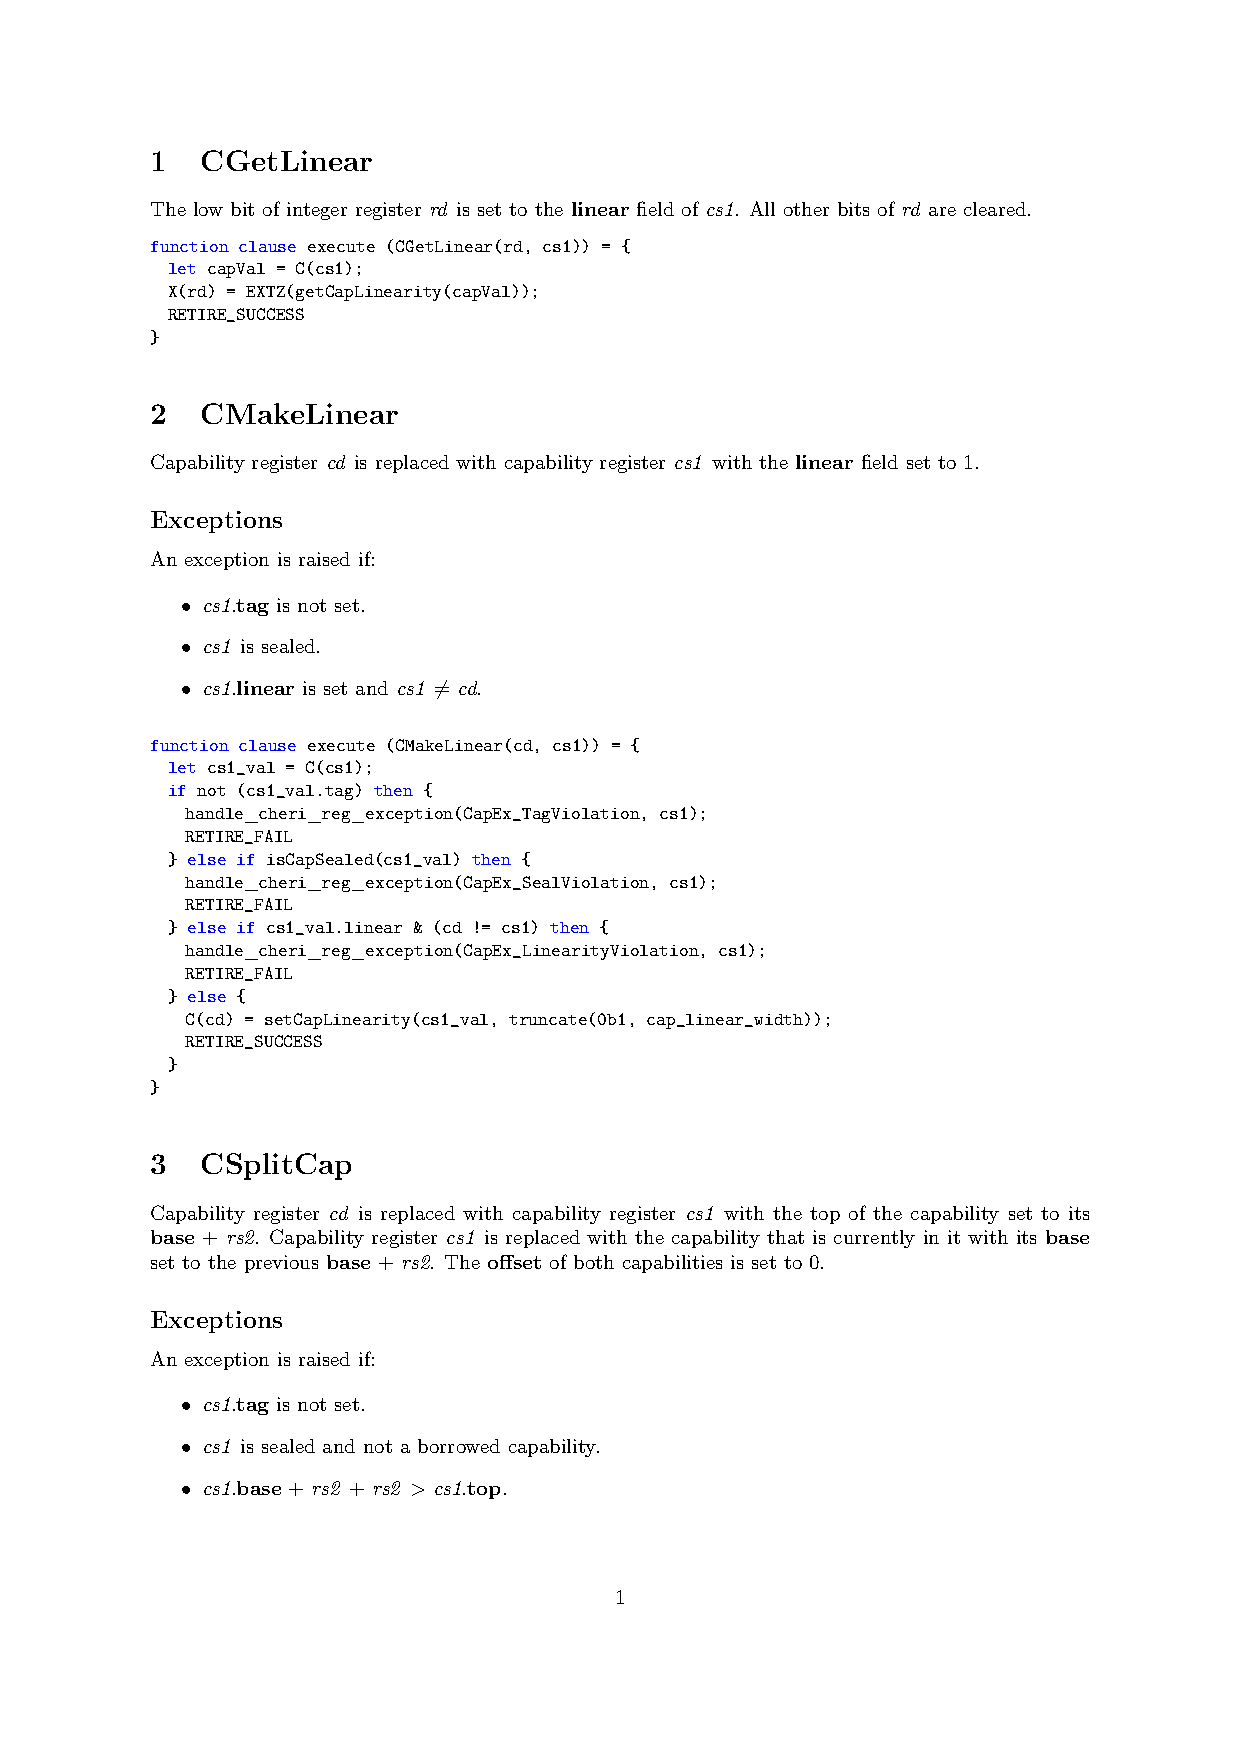
\includepdf[pages=-]{sailcode.pdf}

%%% Local Variables: 
%%% mode: latex
%%% TeX-master: "thesis"
%%% End: 


\backmatter
% The bibliography comes after the appendices.
% You can replace the standard "abbrv" bibliography style by another one.
\bibliographystyle{abbrv}
\bibliography{references}

\end{document}

%%% Local Variables: 
%%% mode: latex
%%% TeX-master: t
%%% End: 
